\chapter{Model and implementation}
\label{ch:model}
%\input{control}

\section{Input Model}

(Coming later)
 
 \subsection{Model of Price Curve}
 Non-parametric approach to model the electricity price curve \cite{Electricity-price-curve}.
 \subsection{Impacts of Renewable Penetration}
 \subsubsection{Renewable support schemes}
 \begin{itemize}
 	\item Feed-in tariff
 	\item Feed-in premium
 	\item Tendering
 	\item Green certificate: Australia, US
 \end{itemize}
 \textbf{Germany}
 \begin{itemize}
 	\item 2000: Feed-in tariff
 	\item 2012: Feed-in tariff + Fixed premium
 	\item 2014: Feed-in tariff + Fixed premium + Tendering pilot
 	\item 2016: Tendering
 \end{itemize}
 \newpage
 
\section{Optimization}
In order to quantify the up bound of value from flexibility, we set up a optimization program, which is designated to answer the question: with certain amount of flexible assets, how much revenue can be captured in a certain market, by optimally scheduling the trades in energy and ancillary services markets.  As is shown by \ref{fig:optimization}, inputs of the optimization come from both the market and technology side. On the market aspect, the price and load data in day-ahead and real-time market, as well as the payments and volume in ancillary service markets are provided, either from historical data or constructed by our own with a model. On the technology side, we first examined two technologies, i.e. Energy Storage Systems (ESS) and Electric Vehicles (EV). The size of flexibility source (defined by charging rate for ESS or number of EVs, for example)is identified and the technical parameters like efficiencies are given. With these inputs, the optimization program will find the optimal utilization scheme of the asset and quantify the revenue created from the market.

 \begin{figure}[h!]
 	\label{fig:optimization}
 	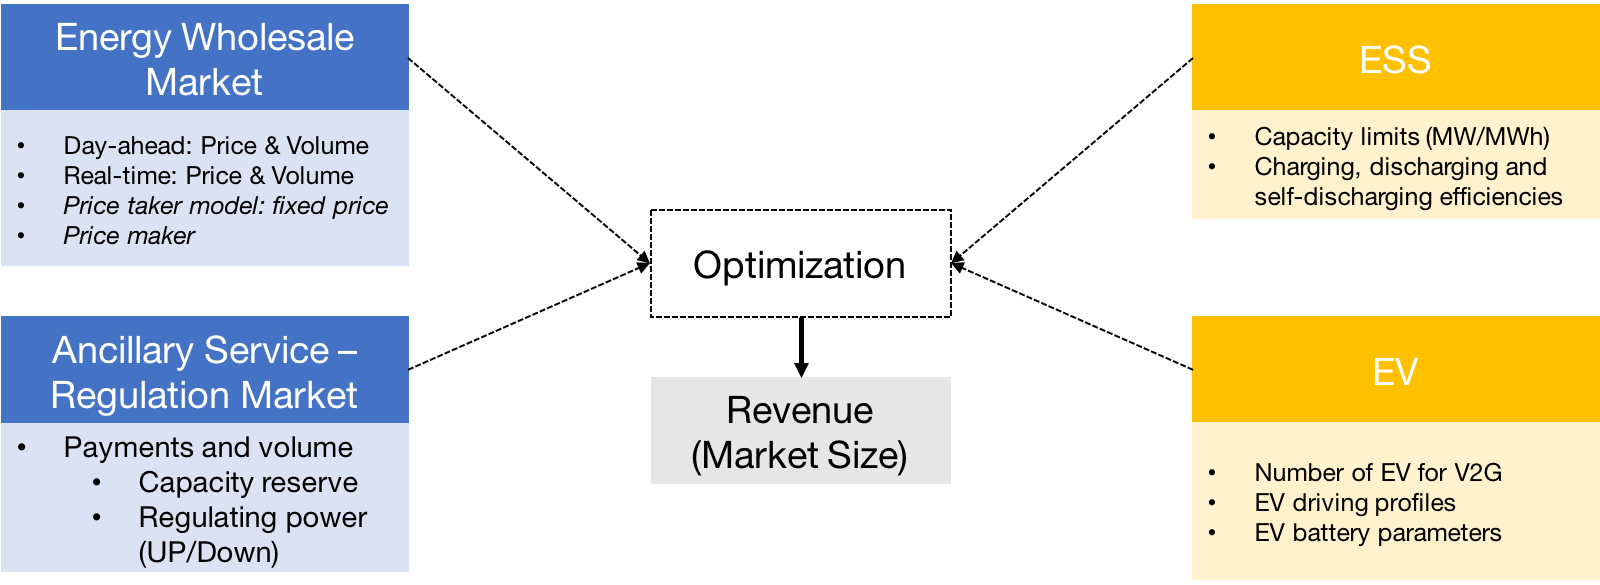
\includegraphics[scale=0.4]{Optimization}
 	\caption{Schematic chart for the optimization program}\
 \end{figure}

The optimization can be carried out globally by taken all variables in \ref{fig:optimization} into a single program, or separately with certain combinations, e.g. ESS in day-ahead market, ESS \& EV in day-ahead market, EV in day-ahead \& real-time \& ancillary service market, etc.

Due to the distinguishing natures of two technologies, we would formulate and run the optimization separately for ESS and EV.  

\subsection{Energy Storage Systems (ESS)} \label{sec:opt-ESS}

\subsubsection{Objective Function}
The revenue of a energy storage system is nothing but the value obtained by selling net of the cost of buying energy in the markets. The objective function that is to maximize the revenue is formulated as \ref{eq:obj-ess}.

\begin{equation}
\label{eq:obj-ess}
\begin{aligned}
& \underset{d_t^{DA}, c_t^{DA}, d_t^{RT}, c_t^{RT}, r_t}{\text{maximize}}
& & \sum_t^{t \in T} \mathrm{Revenue_t} \\
& & &= \sum_t^{t \in T} [p_t^{DA} (d_t^{DA}-c_t^{DA}) + p_t^{RT} (d_t^{RT}-c_t^{RT})  \\
& & &    + (p_t^r+p_t^{RU} \delta_t^{RU}-p_t^{RD} \delta_t^{RD}) r_t] \Delta t \\
\end{aligned}
\end{equation}

The variables to be optimized are the discharging/ charging rate for selling/ buying in day-ahead \& real-time markets and the reserved capacity in ancillary services market at each time point.

\subsubsection{Constraints}
We categorize the constraints to two sets, i.e. technical and market constraints.

\textbf{Technical Constraints}

The technical constraints are associated with the dynamics of the flexible asset, which are determined by their technical nature. For Energy Storage Systems (ESS), these include:

The state equation for the ESS, where the charging/ discharging and self-discharging are modeled:
\begin{equation}
\label{eq:state-ess}
S_t = \eta_s S_{t-1} + [\eta_c(c_t^{DA}+c_t^{RT}+\delta^{RD}_t r_t)  - (1/\eta_d)(d_t^{DA}+d_t^{RT}+\delta^{RU}_t r_t)]\Delta t
\end{equation}

The grid operator is responsible for controlling regulation. The service is called upon for multiple times per day with varying power. Referring to similar works \cite{Berrada2016} \cite{Byrne2012}, the actual dispatched energy for this service is the amount of capacity procured by the grid operator multiplied by a fraction of the actual amount of regulation called in real-time. We use $\delta^{RU}$ and $\delta^{RD}$ to represent the fractions for regulation up and relation down respectively. 

 $\delta^{RU}$ and $\delta^{RD}$ can be assumed to be around 0.1 according to \cite{Berrada2016} \cite{Byrne2012}. However, there exists the risk that the reserved capacity would be fully called by the system operator, which are not considered in the previous works. In order to incorporate the risk, we induce a risk factor $\delta_r$ to cover the additional reserved margin to provide regulation energy. Thereby the state of charge is constrained as:
 
\begin{equation}
\label{eq:limit-state}
	(1/\eta_d)\delta_r r_t \Delta t \leq S_t \leq S_t^{max} - \eta_c\delta_r r_t \Delta t
\end{equation}

The charging/ discharging rates are limited by the capacity:
\begin{equation}
\label{eq:limit-discharge-rate}
d_t^{DA} + d_t^{RT} +\delta^{RU}_t r_t \leq d_t^{max}
\end{equation}

\begin{equation}
\label{eq:limit-charge-rate}
c_t^{DA} + c_t^{RT} +\delta^{RD}_t r_t \leq c_t^{max}
\end{equation}

Non-negativity conditions:
\begin{equation}
d_t^{DA}, c_t^{DA}, d_t^{RT}, c_T^{RT}, r_t \geq 0
\end{equation}

All the constraints above shall be valid at any time:
\begin{equation*}
\forall t \in [1, 2, ..., T]
\end{equation*}

\textbf{Market Constraints}

Aside of the technology, there are constraints due to the market conditions:

In day-ahead market, the net load (minus the flexible power) that is supplied by generations shall be non-negative and below a up limit:
\begin{equation}
\label{eq:market-da-low}
l_t^{DA} - d_t^{DA} + c_t^{DA} \geq 0
\end{equation}

\begin{equation}
\label{eq:market-da-high}
l_t^{DA} - d_t^{DA} + c_t^{DA} \leq l_{max}^{DA}
\end{equation}

Here we take a maximum load over a certain period and assume the shifted load shall not go beyond that value.

In real-time market, the similar constraints exist: 

\begin{equation}
\label{eq:market-rt-low}
l_t^{RT} - d_t^{RT} + c_t^{RT} \geq 0
\end{equation}

\begin{equation}
\label{eq:market-rt-high}
l_t^{RT} - d_t^{RT} + c_t^{RT} \leq l_{max}^{RT}
\end{equation}

In ancillary service - regulation control market:
\begin{equation}
\label{eq:market-as-high}
r_t \leq r_t^{max}
\end{equation}

Besides, since we couple the real-time and day-ahead markets in our optimization, it is likely visual biddings that arbitrage between the real-time and day-ahead markets may take this advantage of perfect predictability. Visual bids exist ((8\% to 12\% in MISO \cite{Limit-visual-bid})) and are allowed in many markets because it increases market efficiencies in many aspects. However, this value shall not be accounted for the value created by flexibility because the assets are not really utilized. In case the buying/ selling in real-time market offset the selling/ buying in day-ahead market, the \eqref{eq:limit-state} becomes slack. In order to overcome this issue, we need to ensure that trading in the day-ahead market shall always fulfill the limit for \eqref{eq:limit-state}, without know the optimal operation in the real-time price in the next day.

\begin{equation}
\label{eq:virtual-bidding}
0 \leq  \eta_s S_{t-1} + (\eta_c c_t^{DA} - (1/\eta_d)d_t^{DA})\Delta t \leq S_t^{max}
\end{equation}

Again, all market constraints shall be fulfilled at any time point:

\begin{equation*}
\forall t \in [1, 2, ..., T]
\end{equation*}

\subsection{Electric Vehicles (EVs)}
EVs are being implemented used as a grid resource with vehicle-to-grid (V2G) technologies. In this study we conceive EVs as a dynamics ESS with variable parameters as the number of EVs connected in the grid changes temporally.

\subsubsection{Objective Function}
The objective function for ESSs \ref{eq:obj-ess} can be applied for EVs as well. However, the revenue defined by \eqref{eq:obj-ess} implicitly contains the cost for charging the EVs which shall be added back. The cost for charging the EVs can be computed separately with a original scheme. In order to simplify the problem, we assume with the original schedule, the EVs are to be charged immediately after it is connected to the grid and all charging take $H$ hours to complete. 

Thereby, the number of EV being charged can be computed as
\begin{equation}
N_t^{EV-c} = (n_t^+ + n_{t-1}^+ + \dots + n_{t-H}^+)
\end{equation}

The total electricity consumed to charge the EV with the optimized scheme can be computed as:

\begin{equation}
E^{EV-c} = \sum_{t}^{t \ in T}[(c_t^{DA}+c_t^{RT}+\delta^{RD}_t r_t)  - (d_t^{DA}+d_t^{RT}+\delta^{RU}_t r_t)]\Delta t
\end{equation}

Assuming the total electricity for charging the EVs remains unchanged, the cost of charging with original scheme can be computed as
\begin{equation}
Cost_t = p_t \dfrac{E^{EV-c}}{\sum N_t^{EV-c} } N_t^{EV-c} 
\end{equation}

In computation, either day-ahead or real-time price can be used to determine $p_t$.
\subsubsection{Constraints}
EV fleet can be conceived as a ESS but with dynamic capacity. In order to model the process, we introduce variables $n_t^+$ and $n_t^-$ to define the number of EVs connected to and disconnected from the grid, and $N_t$ as the number EVs being connected to the grid. Thereby the state equation becomes:
\begin{equation}
\label{eq:state-EV}
S_t = \eta_s S_{t-1} + [\eta_c(c_t^{DA}+c_t^{RT}+\delta^{RD}_t r_t)  - (1/\eta_d)(d_t^{DA}+d_t^{RT}+\delta^{RU}_t r_t)]\Delta t + s^+ n_t^+ - s^- n_t^-
\end{equation}

\begin{equation}
\label{eq:state-EV-nb}
n_t = n_{t-1} +n_t^+ - n_t^-
\end{equation}

the term $s$ is the maximum energy stored in a single EV and we assume the EVs disconnected shall be full charged while the EV entered.

The constraints for charging/ discharging rates formulated as \eqref{eq:limit-charge-rate} and \eqref{eq:limit-discharge-rate} are still valid, but the terms $d_t^{max}$ and $c_t^{max}$ are no longer constant but proportional to $N_t$.

Technology constraints are same as in section \ref{sec:opt-ESS}.


\section{Implementation}
\label{Implementation}

\subsection{Optimization}
\subsubsection{Energy Storage Systems}
The optimizing variable $X$ is formulated as 
\[
X = 
\begin{bmatrix}
	D^{DA} \\
	C^{DA} \\
	D^{RT} \\
	C^{RT} \\
	R \\
\end{bmatrix}
=
\begin{bmatrix}
	d_1^{DA} \\
	\vdots \\
	d_T^{DA} \\ 
	c_1^{DA} \\
	\vdots \\
	c_T^{DA} \\ 
	d_1^{RT} \\
	\vdots \\
	d_T^{RT} \\ 
	c_1^{RT} \\
	\vdots \\
	c_T^{RT} \\
	r_1 \\
	\vdots \\
	r_T
\end{bmatrix}
\]
In order to implement the equality constraint (state equation), we introduce a matrix $M_s$:
\[
M_s
=
\begin{bmatrix}
\eta_s^0 & 0 & 0 & 0 & \dots & 0 \\
\eta_s^1 & \eta_s^0 & 0 & 0 & \dots & 0 \\
\eta_s^2 & \eta_s^1 & \eta_s^0 & 0 & \dots & 0 \\
\vdots & \vdots & \vdots & \vdots & \ddots & \vdots \\
\eta_s^{T-1} & \eta_s^{T-2} & \eta_s^{T-3} & \eta_s^{T-4} & \dots & \eta_s^0 \\
\end{bmatrix}
\]
Then the state equation for \eqref{eq:state-ess} can be represented in matrix format as:
\begin{equation*}
S = \eta_s M_s S_0 + [-\frac{1}{\eta_d}M_s | \eta_c M_s | -\frac{1}{\eta_d}M_s | \eta_c M_s | -\frac{1}{\eta_d}  \delta^{RU} M_s + \eta_c \delta^{RD} M_s ] X \Delta t
\end{equation*}
\[
S = 
\begin{bmatrix}
S_1 & S _2 & S_3 & \dots & S_T
\end{bmatrix} ^ {T}
\]

\[
S_0 = 
\begin{bmatrix}
S_0 & S _0 & S_0 & \dots & S_0
\end{bmatrix} ^ {T}
\]

Thereby, the inequality constraint for the state \eqref{eq:limit-state} can be formulated as:

\begin{equation*}
- [-\frac{1}{\eta_d}M_s | \eta_c M_s | -\frac{1}{\eta_d}M_s | \eta_c M_s | -\frac{1}{\eta_d}  (\delta^{RU} + \delta^r) M_s + \eta_c \delta^{RD} M_s ] X \Delta t \leq \eta_s M_s S_0 
\end{equation*}

and 

\begin{equation*}
[-\frac{1}{\eta_d}M_s | \eta_c M_s | -\frac{1}{\eta_d}M_s | \eta_c M_s | -\frac{1}{\eta_d}  \delta^{RU} M_s + \eta_c (\delta^{RD}+\delta^r) M_s ] X \Delta t \leq S_{max} - \eta_s M_s S_0
\end{equation*}

Inequality constraint \eqref{eq:limit-discharge-rate}:
\begin{equation*}
[I_T | O_T | I_T | O_T | \delta_t^{RU}I_T]X \leq D^{max}
\end{equation*}

Inequality constraint \eqref{eq:limit-charge-rate}:
\begin{equation*}
[O_T | I_T | O_T | I_T | \delta_t^{RD}I_T]X \leq C^{max}
\end{equation*}

$I_T$ is a T-by-T identity matrix while $O_T$ is a T-by-T zero matrix. 

Inequality constraint \eqref{eq:market-da-low}
\begin{equation*}
[I_T | -I_T | O_T | O_T | O_T]X \leq L^{DA}
\end{equation*}

Inequality constraint \eqref{eq:market-da-high}
\begin{equation*}
[-I_T | I_T | O_T | O_T | O_T]X \leq L_{max}^{DA} - L^{DA}
\end{equation*}

Inequality constraint \eqref{eq:market-rt-low}
\begin{equation*}
[O_T | O_T | I_T | -I_T | O_T]X \leq L^{RT}
\end{equation*}

Inequality constraint \eqref{eq:market-rt-high}
\begin{equation*}
[O_T | O_T | -I_T | I_T | O_T]X \leq L_{max}^{RT} - L^{RT}
\end{equation*}

Inequality constraint \eqref{eq:market-as-high}
\begin{equation*}
[O_T | O_T | O_T | O_T | I_T]X \leq R_{Max}
\end{equation*}

Inequality constraint \eqref{eq:virtual-bidding}
\begin{equation*}
-[-\frac{1}{\eta_d}M_s | \eta_c M_s| O_T | O_T | O_T]X \leq \eta_s M_s S_0
\end{equation*}

\subsubsection{Electric Vehicles}

Analogous to ESS, the state equation for EVs \eqref{eq:state-EV} can be formulated as:
\begin{equation*}
S = \eta_s M_s S_0 + [-\frac{1}{\eta_d}M_s | \eta_c M_s | -\frac{1}{\eta_d}M_s | \eta_c M_s | -\frac{1}{\eta_d}  \delta^{RU} M_s + \eta_c \delta^{RD} M_s ] X  + M_s s^+ N^+ - M_s s^- N^-
\end{equation*}

The number of EVs on-line can be represented as:

\[
N = 
\begin{bmatrix}
1& 0 & 0 & \dots & 0 \\
0& 1 & 0 & \dots & 0 \\
\vdots & \vdots & \vdots & \ddots & \vdots \\
0& 0 & 0 & \dots & 1 \\
\end{bmatrix}
\begin{bmatrix}
n_0 \\
n_0 \\
\vdots \\
n_0 \\
\end{bmatrix}
+
\begin{bmatrix}
1& 0 & 0 & \dots & 0 \\
1& 1 & 0 & \dots & 0 \\
\vdots & \vdots & \vdots & \ddots & \vdots \\
1& 1 & 1 & \dots & 1 \\
\end{bmatrix}
\begin{bmatrix}
n_1^+ \\
n_2^+  \\
\vdots \\
n_T^+  \\
\end{bmatrix}
-
\begin{bmatrix}
1& 0 & 0 & \dots & 0 \\
1& 1 & 0 & \dots & 0 \\
\vdots & \vdots & \vdots & \ddots & \vdots \\
1& 1 & 1 & \dots & 1 \\
\end{bmatrix}
\begin{bmatrix}
n_1^-  \\
n_2^- \\
\vdots \\
n_T^- \\
\end{bmatrix}
\]

\begin{equation*}
N = I_T N_0 + L_T N^+ - L_T N^-
\end{equation*}



The inequality constraints for the state of EV:

\begin{equation*}
- [-\frac{1}{\eta_d}M_s | \eta_c M_s | -\frac{1}{\eta_d}M_s | \eta_c M_s | -\frac{1}{\eta_d}  (\delta^{RU} + \delta^r) M_s + \eta_c \delta^{RD} M_s ] X \Delta t \leq \eta_s M_s S_0 + M_s s^+ N^+ - M_s s^- N^-
\end{equation*}

and 

\begin{equation*}
[-\frac{1}{\eta_d}M_s | \eta_c M_s | -\frac{1}{\eta_d}M_s | \eta_c M_s | -\frac{1}{\eta_d}  \delta^{RU} M_s + \eta_c (\delta^{RD}+\delta^r) M_s ] X \Delta t \leq s_{max} N - \eta_s M_s S_0 - M_s s^+ N^+ + M_s s^- N^-
\end{equation*}

Inequality constraint \eqref{eq:limit-discharge-rate}:
\begin{equation*}
[I_T | O_T | I_T | O_T | \delta_t^{RU}I_T]X \leq d^{max} N
\end{equation*}

Inequality constraint \eqref{eq:limit-charge-rate}:
\begin{equation*}
[O_T | I_T | O_T | I_T | \delta_t^{RD}I_T]X \leq c^{max} N
\end{equation*}

The market constraints are identical as for ESSs.
 
 The terms $N^+$ and $N^+$ are determined by the EV driving profiles. Based on real-world data \cite{Transport-data} we preliminarily determined the profiles of $N^+$ and $N^+$ in a single day as Figure \ref{fig:EV-nb-inout}:
 \begin{figure}[h!]
 	\label{fig:EV-nb-inout}
 	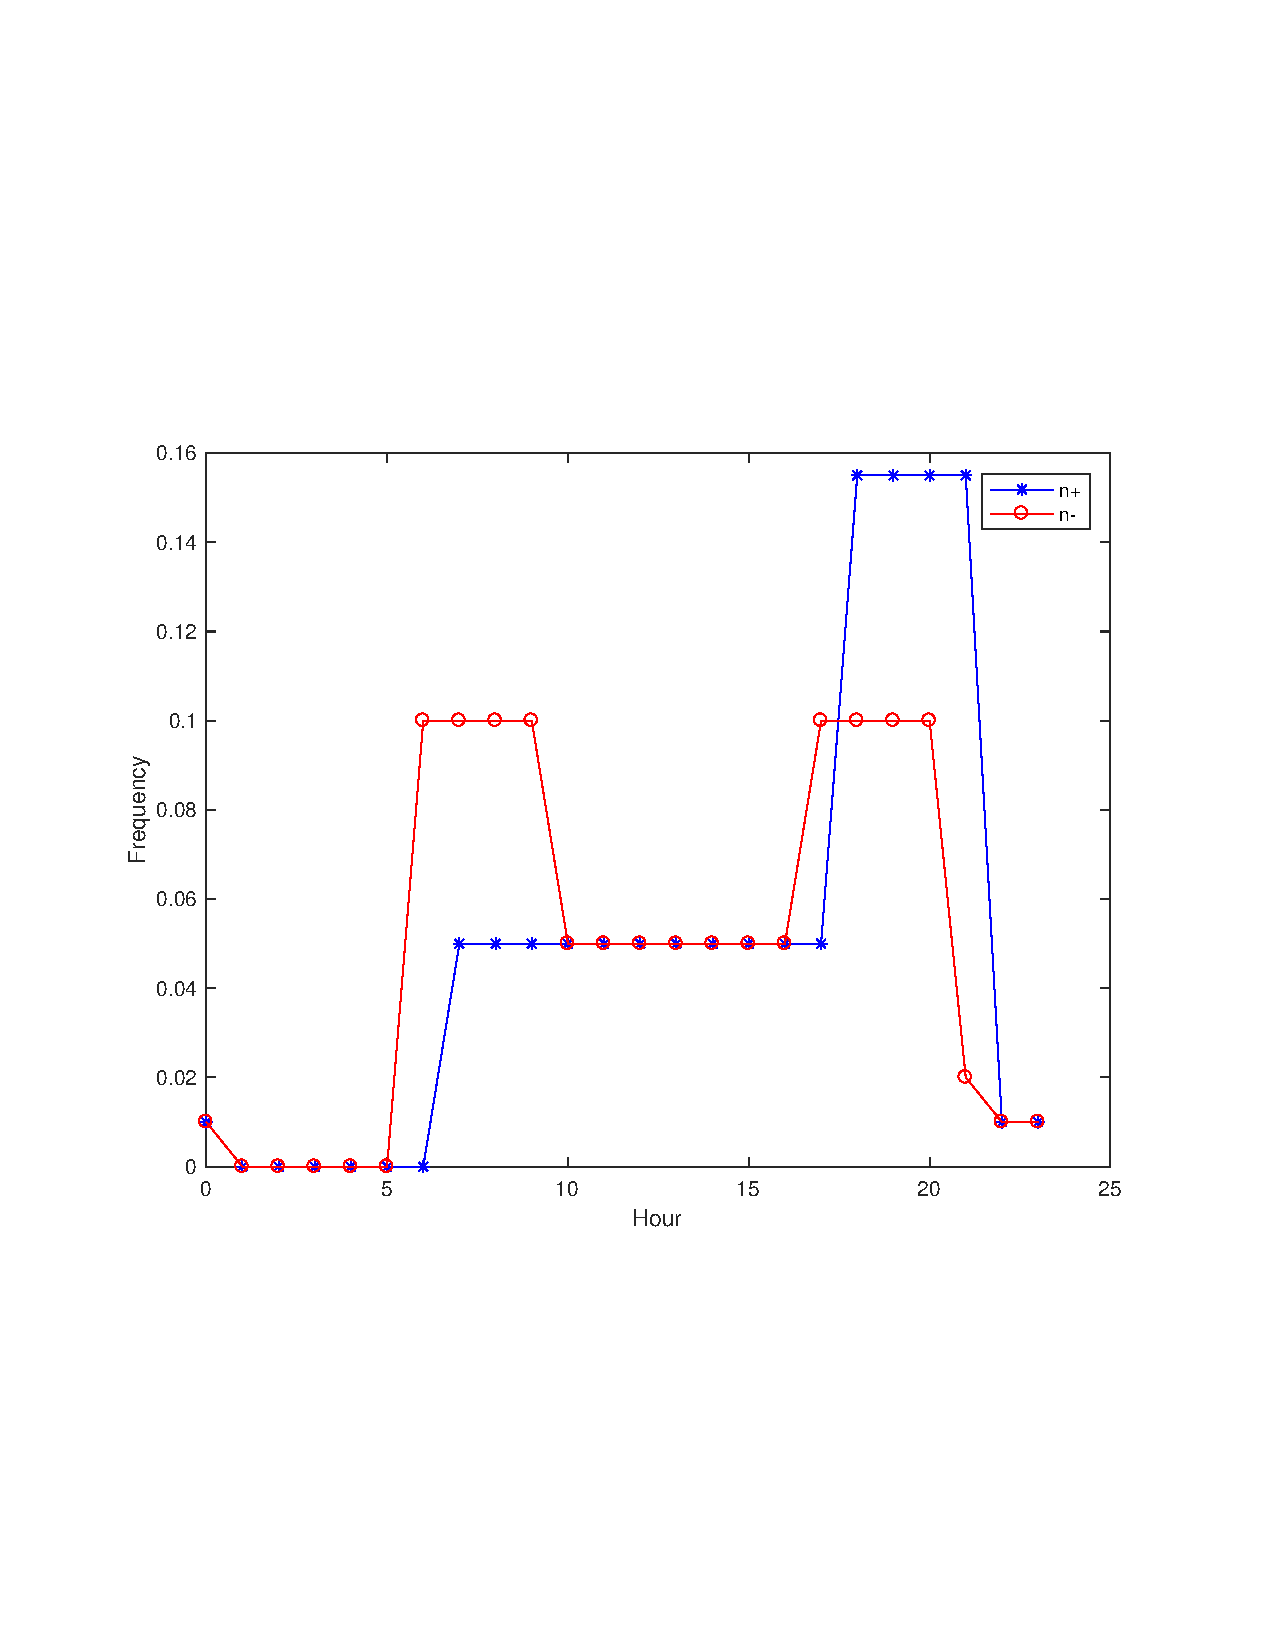
\includegraphics[scale=0.6]{EV_state_nb_inout}
 	\caption{Profiles of EV connected to $N^+$ and disconnected from $N^+$ grid in 24-h}
 \end{figure}
 
 The number of EVs on-line can be thus calculated (Figure \ref{fig:EV-nb}):
 \begin{figure}[h!]
 	\label{fig:EV-nb}
 	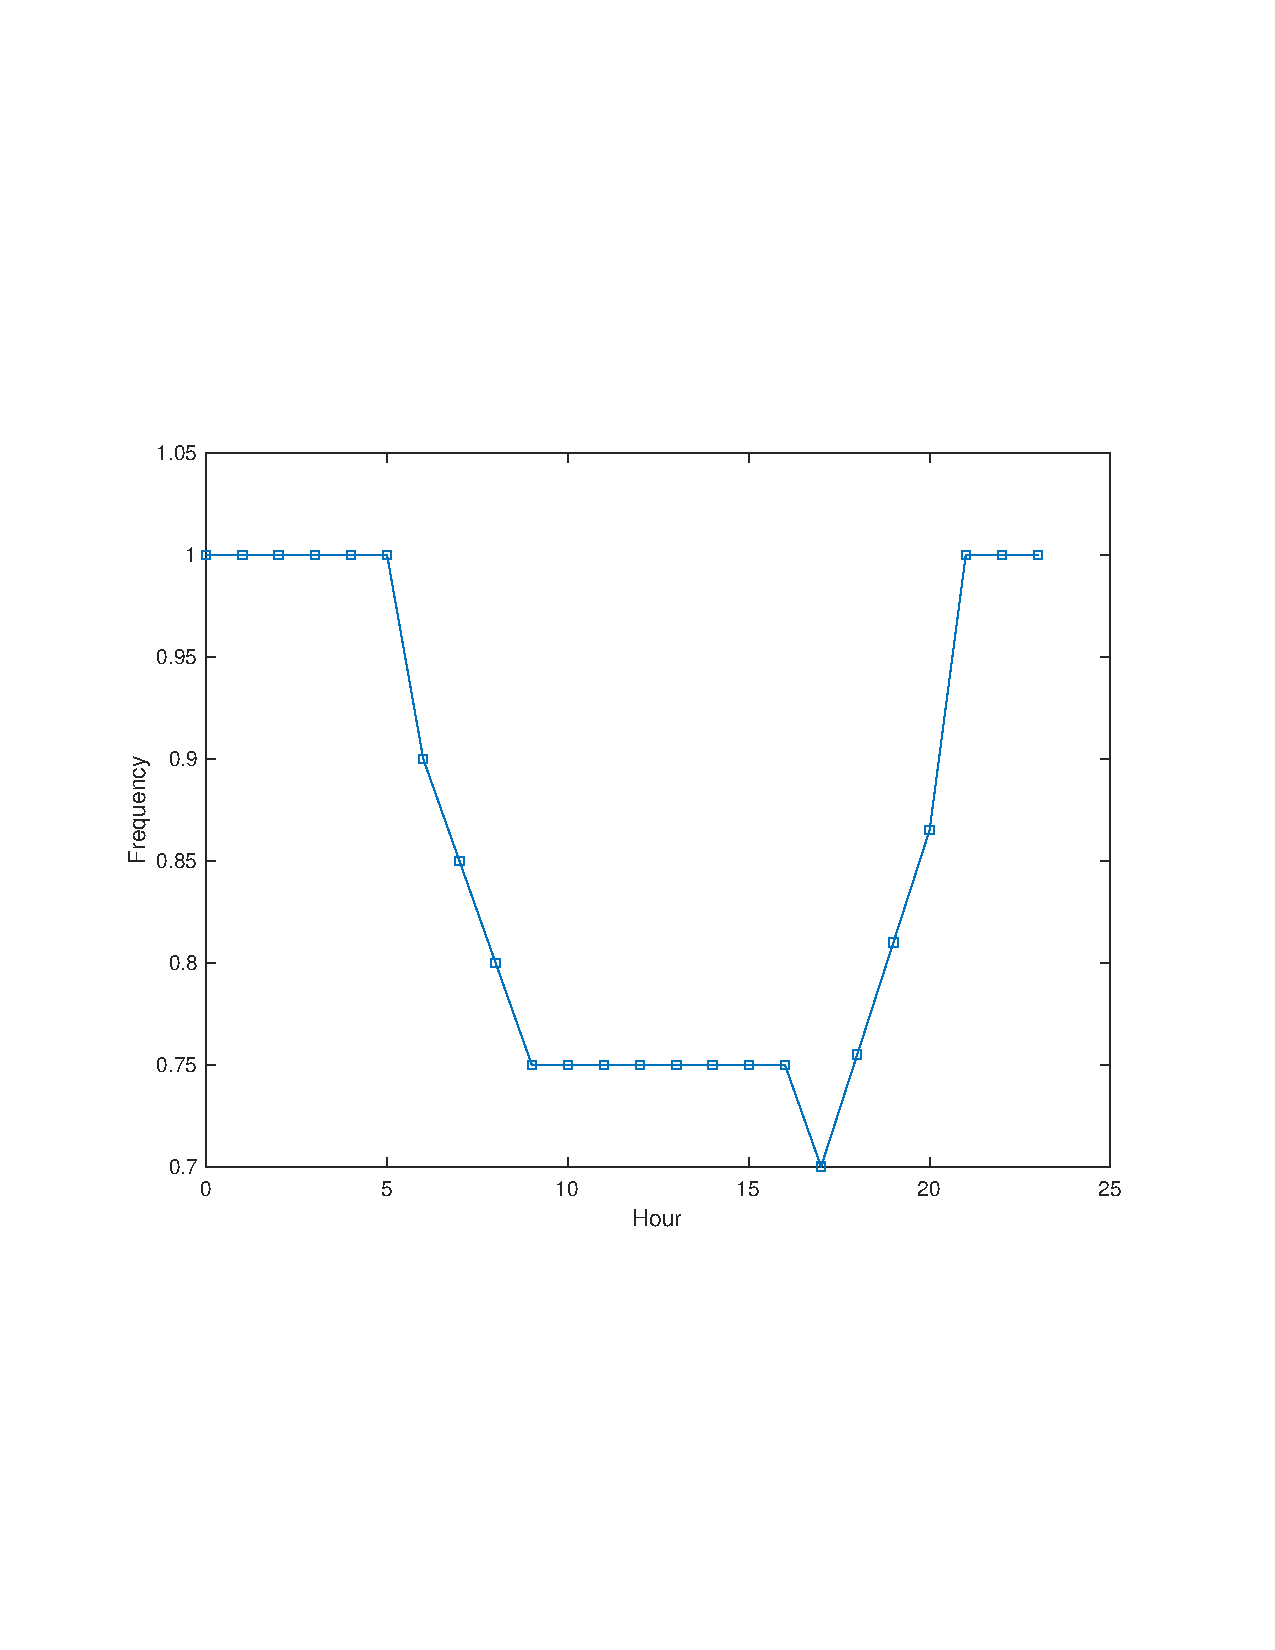
\includegraphics[scale=0.6]{EV_state_nb}
 	\caption{Profiles of on-line EVs number $N$ in 24-h}
 \end{figure}